\chapter{Conclusions}

\section{Performance Profile plots}
The Performance Profiler \cite{dolan2002benchmarking} is a tool that facilitates the visualization of comparisons between the results of different algorithms. Depending on the type of algorithm, users can choose to compare various aspects of the results. In our case, when comparing heuristic methods, we are interested in the quality of the solutions found, so we use the solution cost as the metric. Conversely, when comparing exact algorithms, the solutions are always the same (the optimal one), but the focus shifts to the time required to find these solutions.

The performance profile classifies the execution times (or solution costs) based on the success percentage relative to a multiplication factor (ratio). The trend of the performance profile of an algorithm is monotonically increasing. The value for each ratio in the graph represents the percentage of instances that the algorithm solves with that factor compared to the optimum for that case. These graphs are often represented on a logarithmic scale to better highlight differences and achieve a clearer depiction.

The program used to create the performance profiles of the different algorithms is \textit{perprof.py}, developed by D. Salvagnin in 2016 \cite{salvagnin2016performance}.

\section{Heuristic and Metaheuristic methods}
The diagram illustrates the performance of various heuristic and metaheuristic methods for solving the Traveling Salesman Problem (TSP): Nearest Neighbor (NN), NN with 2-opt optimization, NN with Tabu Search, and NN with Variable Neighborhood Search (VNS). The Nearest Neighbor (NN) method is the least effective, with solutions deviating 15-20\% from the optimal cost, as shown by the red curve. Applying 2-opt optimization significantly improves the NN method, achieving solutions within 5\% of the optimal cost, indicated by the blue curve. Both Tabu Search and VNS perform similarly, with solutions within approximately 5\% of the optimal cost, as shown by their overlapping green and purple curves. The 2-opt method alone can nearly match the performance of Tabu Search and VNS, demonstrating its effectiveness. All enhanced methods perform significantly better than the basic NN method, highlighting the importance of optimization techniques in solving the TSP.

The performance profile in Figure \ref{fig:heur_comp} shows that while NN is quick, its performance is suboptimal. Incorporating optimization techniques like 2-opt, Tabu Search, or VNS improves solution quality, reducing the error margin to within 5\% of the optimal solution. The similar performance of 2-opt, Tabu Search, and VNS suggests that the choice among them can be based on computational efficiency or implementation complexity rather than solution quality. This analysis highlights the critical role of optimization in heuristic approaches to combinatorial problems like the TSP.

\begin{figure}[H]
    \centering
    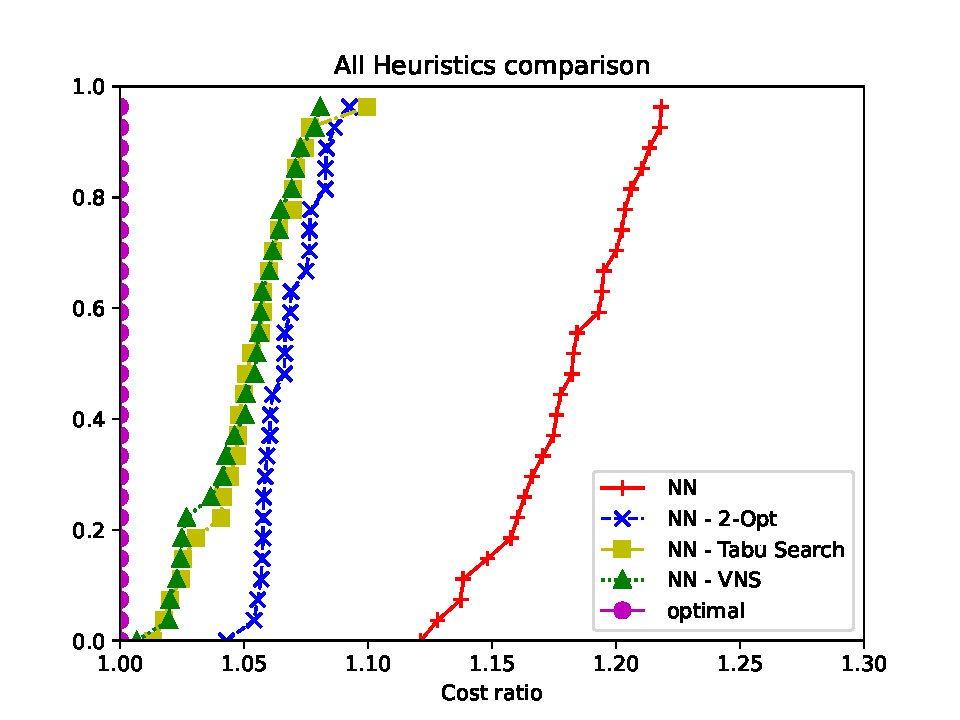
\includegraphics[width=0.7\linewidth]{Immagini/All Heuristics.pdf}
    \caption{Performance profile of all Heuristics methods.}
    \label{fig:heur_comp}
\end{figure}

\section{Exact Methods}
The diagram in Figure \ref{fig:exacts_comp} compares the performance profiles of various exact methods for solving optimization problems, focusing on Benders' decomposition and Branch-and-Cut (B\&C) techniques with different enhancements. Utilizing all available features, such as MIP Start, candidate callback, user-cut callback, and posting, yields the best performance, significantly improving efficiency and solution quality. Even using only the posting method the performance remains highly effective, indicating that it is a particularly powerful technique. The plain B\&C approach with callbacks is effective as much as Benders' loop method, indicating that with our modern computational power even a simpler method can reach very good results.

Overall, the analysis demonstrates that while both Benders' decomposition and B\&C methods are powerful, the strategic use of enhancements like callbacks, MIP start and especially posting significantly influences their performance, making them more efficient and adaptable to real-world scenarios.

\begin{figure}[H]
    \centering
    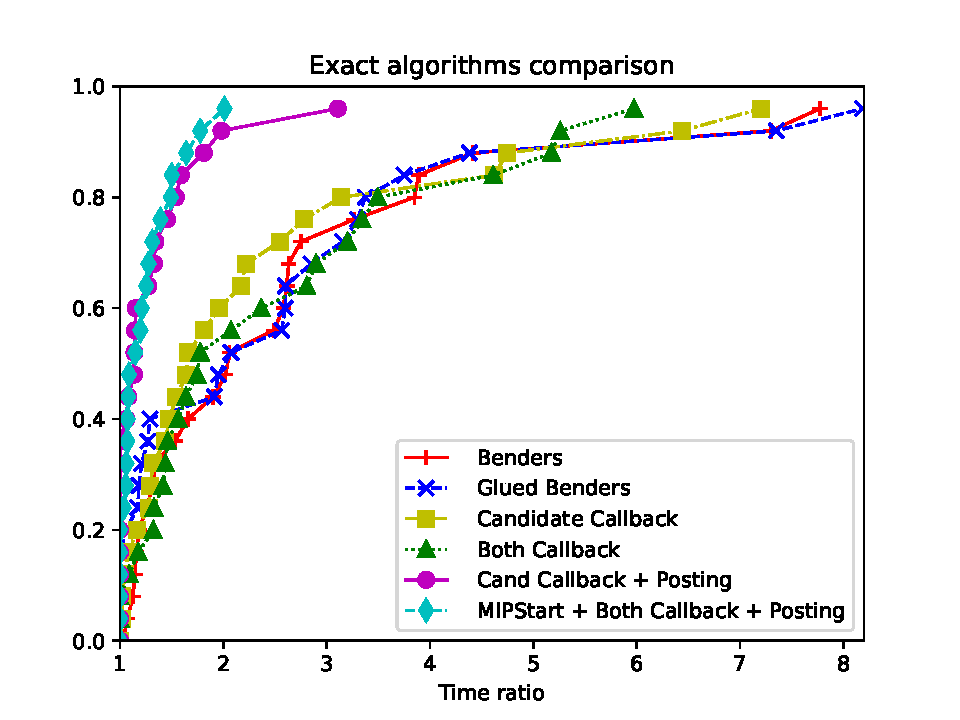
\includegraphics[width=0.7\linewidth]{Immagini/exacts.pdf}
    \caption{Performance profile of all Exact methods.}
    \label{fig:exacts_comp}
\end{figure}

\section{All Heuristics and Matheuristics Methods}
From the results presented in the performance profile in Figure \ref{fig:allheur_comp}, it is evident that matheuristic algorithms significantly outperform both heuristic and metaheuristic algorithms. Within the same category of algorithms, performance differences are almost negligible, except for the Nearest Neighbor (NN) algorithm, which stands out as the least performing among all the considered algorithms. The application of VNS and Tabu Search significantly improves the performance of the Nearest Neighbor algorithm, although the results obtained still do not reach those of Local Branching, which clearly stands out for its better performance. However, Local Branching is consistently outperformed by the Diving algorithm, who seems to be the best one among all the non-exact algorithms.

\begin{figure}[H]
    \centering
    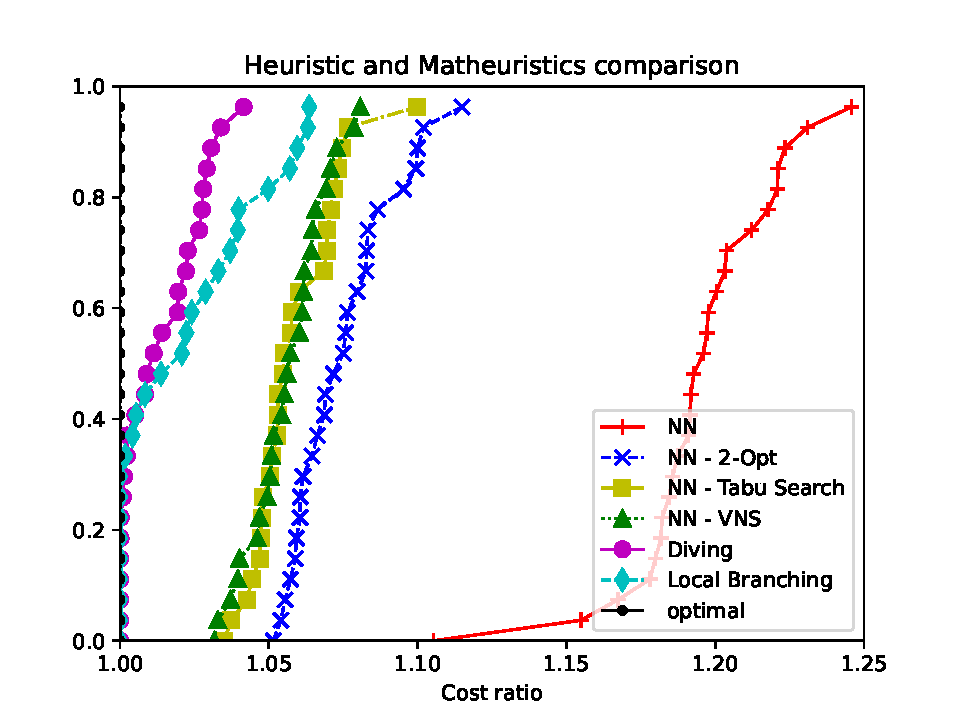
\includegraphics[width=0.7\linewidth]{Immagini/all_heur.pdf}
    \caption{Performance profile of all Heuristic and Matheuristic methods.}
    \label{fig:allheur_comp}
\end{figure}

\section{Final Conclusions}
In conclusion, we can affirm that each algorithm has unique characteristics that make it suitable for specific scenarios and objectives. The choice of the most appropriate algorithm depends on the specific needs of the problem to be solved and the available resources.

If the main goal is to obtain a solution in a short time, even at the cost of not necessarily achieving optimality, heuristic, metaheuristic, and matheuristic algorithms are a valid choice. These approaches use approximation strategies and advanced search techniques to find good solutions quickly, making them ideal for complex problems where speed is essential.

On the other hand, if the aim is to obtain a solution that is as close as possible to the optimum, without considering computation time as a critical factor, exact algorithms are the best choice. These algorithms are designed to explore the entire solution space, thus ensuring the possibility of finding the optimal solution or the one closest to the optimum, albeit at the cost of longer computation times.

In summary, the selection of the algorithm depends on the need to balance solution quality and execution time. Understanding the characteristics and capabilities of each type of algorithm allows for informed decisions and optimization of resources to achieve the desired results in the most efficient way possible.